\section{Experiment: Two particles}
\label{section:experiment:two-particles}

The present experiments study two particles that bump into each other and then
move away because of the spring dashpot forces.
The two particles are represented by 126 triangles. 
We simulate 15,000 time steps.
A contact is detected first in iteration 9,541 and introduces a force making the
two particles to move away from each other. 
The code however still needs another 5 iterations to make the particles be away
from each other more than $\epsilon=10^{-4}$.
If the two particles are compared, this results in 3,944 triangle-triangle
comparisons.
 
The experiments can be rerun with 
{\footnotesize
\begin{verbatim}
./dem-3d-asserts 0.3 0.1 0.02 two-particles-crash 15000 regular-grid 0.0001 \ 
upon-change 0.0

./dem-3d-asserts 0.3 0.1 0.02 two-particles-crash 15000 adaptive-grid 0.0001 \
upon-change 0.0

./dem-3d-asserts 0.3 0.1 0.02 two-particles-crash 15000 reluctant-adaptive-grid \
0.0001 upon-change 0.0
\end{verbatim}
}

{\bf Regular grid.} We obtain a grid with 1,032 vertices. The first 6,334
iterations, we do not perform any contact detection. The subsequent grid
traversals perform all 3,944 comparisons till iteration 12,503. Starting from
time step 12,504, the particles are far away from each other again and we do not
compare anything anymore.

\begin{center}
  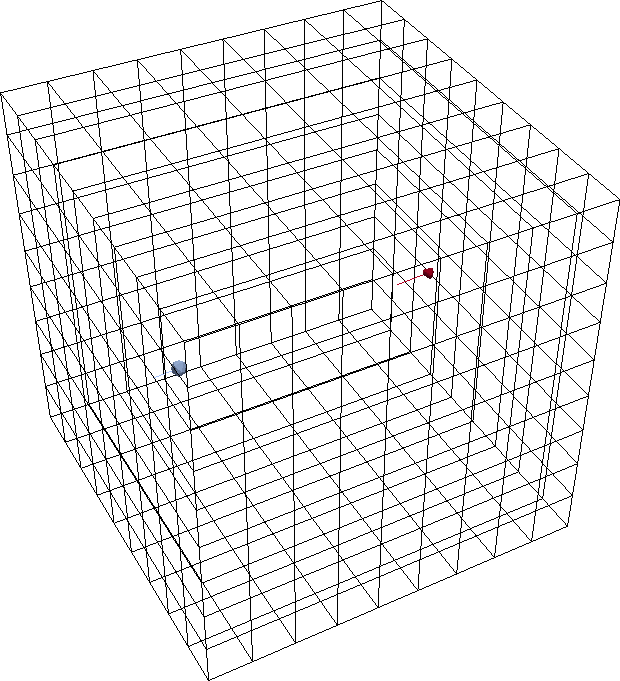
\includegraphics[width=0.3\textwidth]{experiments/two-bodies/visualisation/regular-grid00.png}
  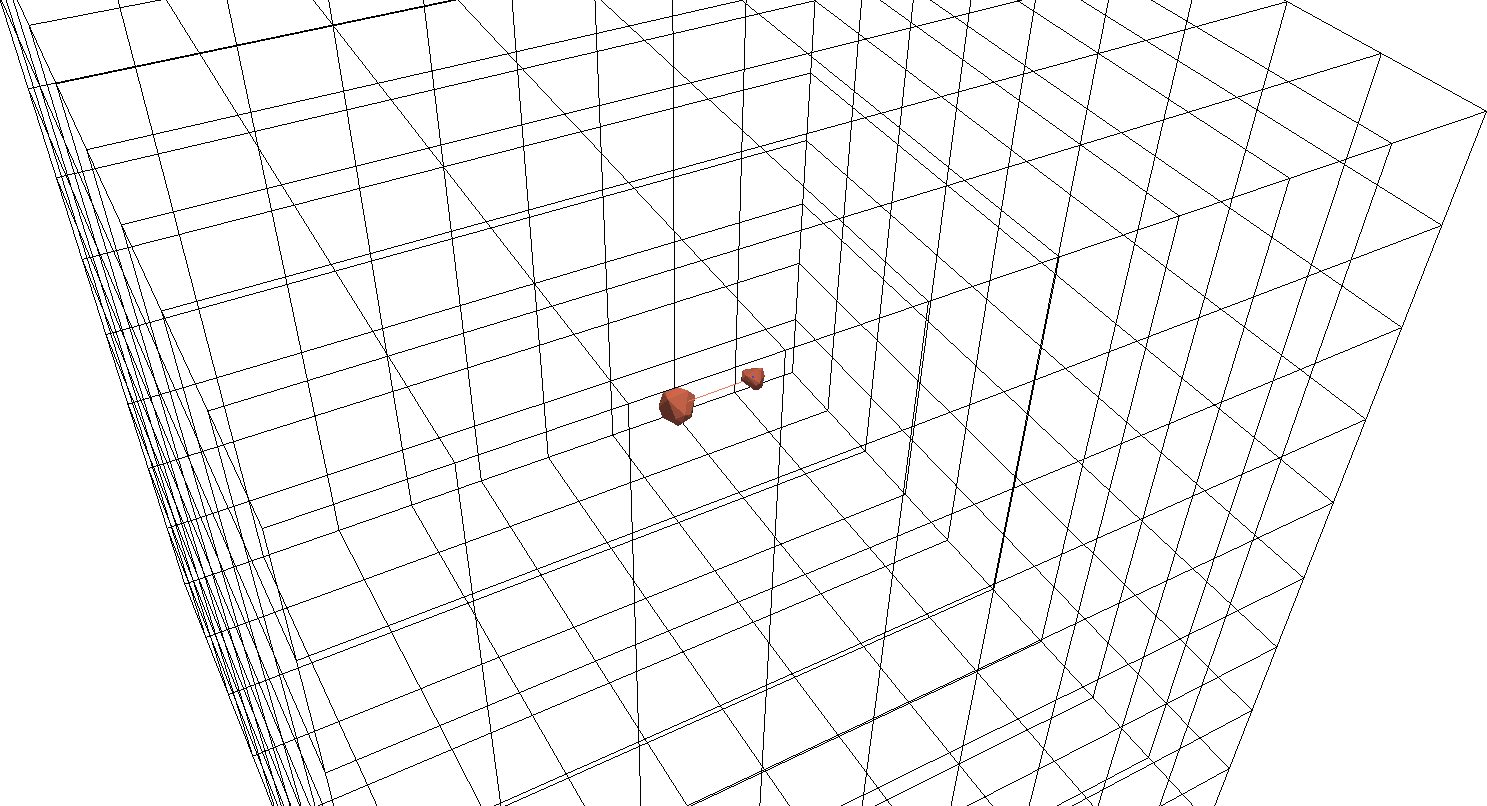
\includegraphics[width=0.3\textwidth]{experiments/two-bodies/visualisation/regular-grid01.png}
  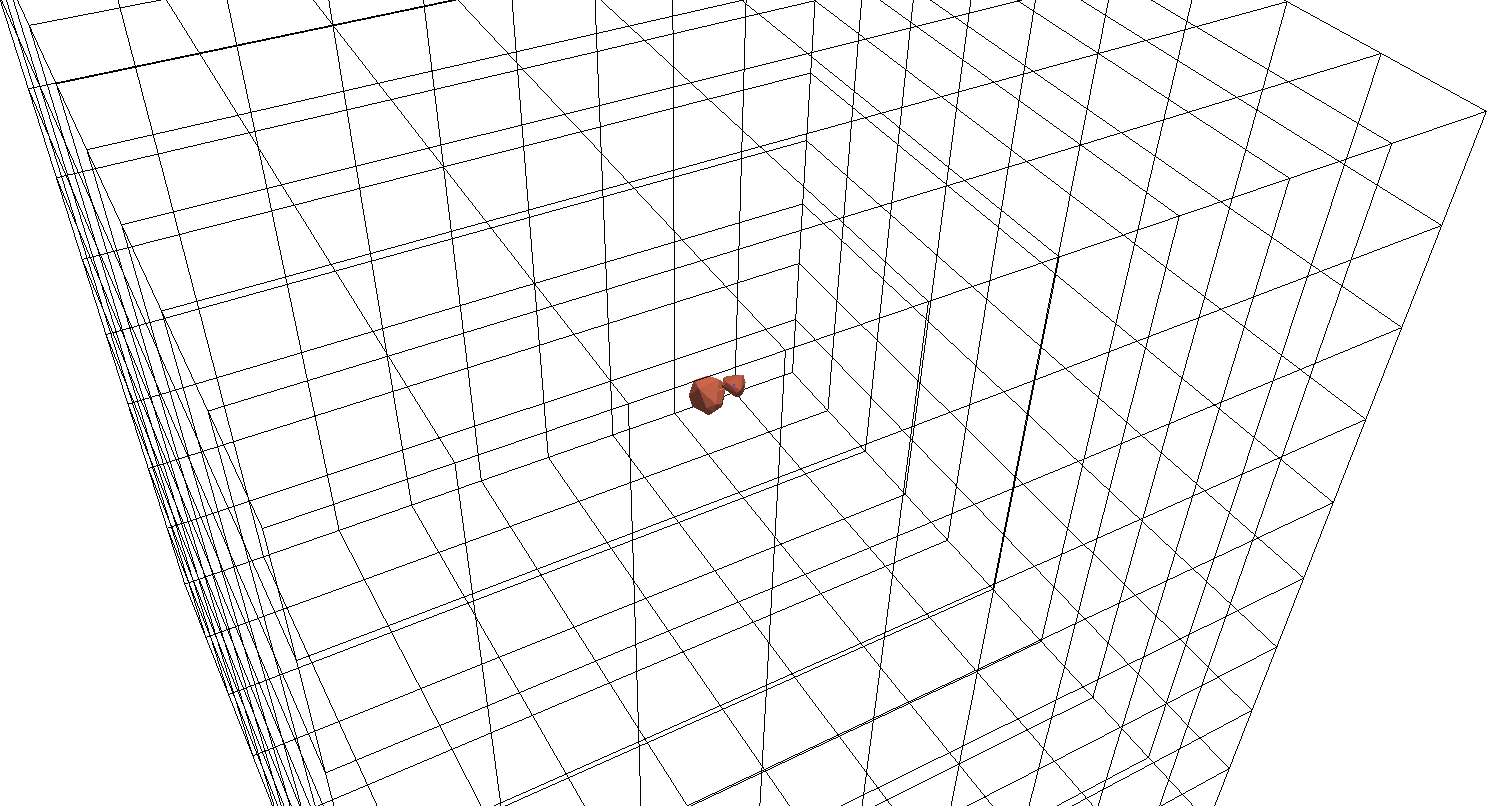
\includegraphics[width=0.3\textwidth]{experiments/two-bodies/visualisation/regular-grid02.png}
\end{center}


{\bf Adaptive grid.} We obtain a grid with 747 vertices. Only few iterations
(when one particle enters a neighbouring region) make the number increase to
980, but these grids are immediately after reduced to 747 again.
The first 8,556 iterations, we do not perform any contact detection. The
subsequent grid traversals perform all 3.944 comparisons.
In iteration 9,539 we detect contact and the particles start to move away
from each other, but we continue to check for further contacts till iteration
10,415.
From here on, the particles are far away from each other again
and we do not compare anything anymore.

% \begin{center}
%   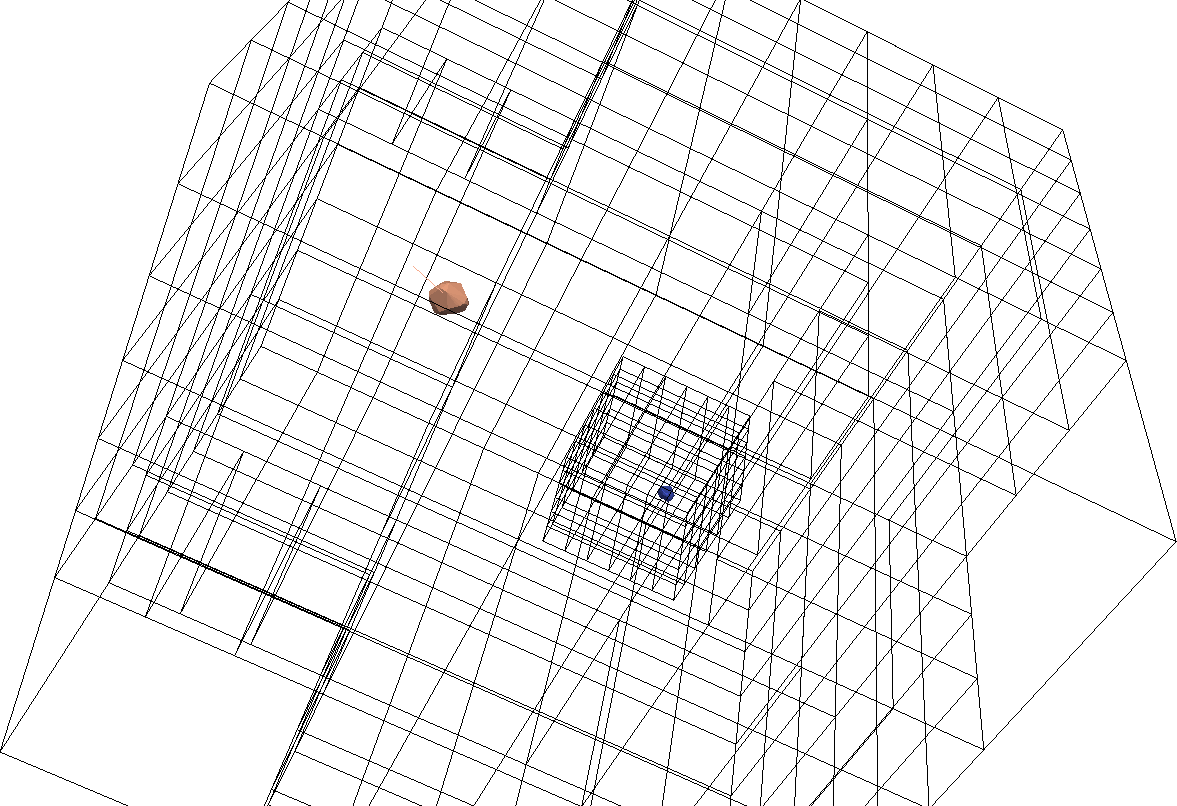
\includegraphics[width=0.3\textwidth]{experiments/two-bodies/visualisation/adaptive-grid00.png}
%   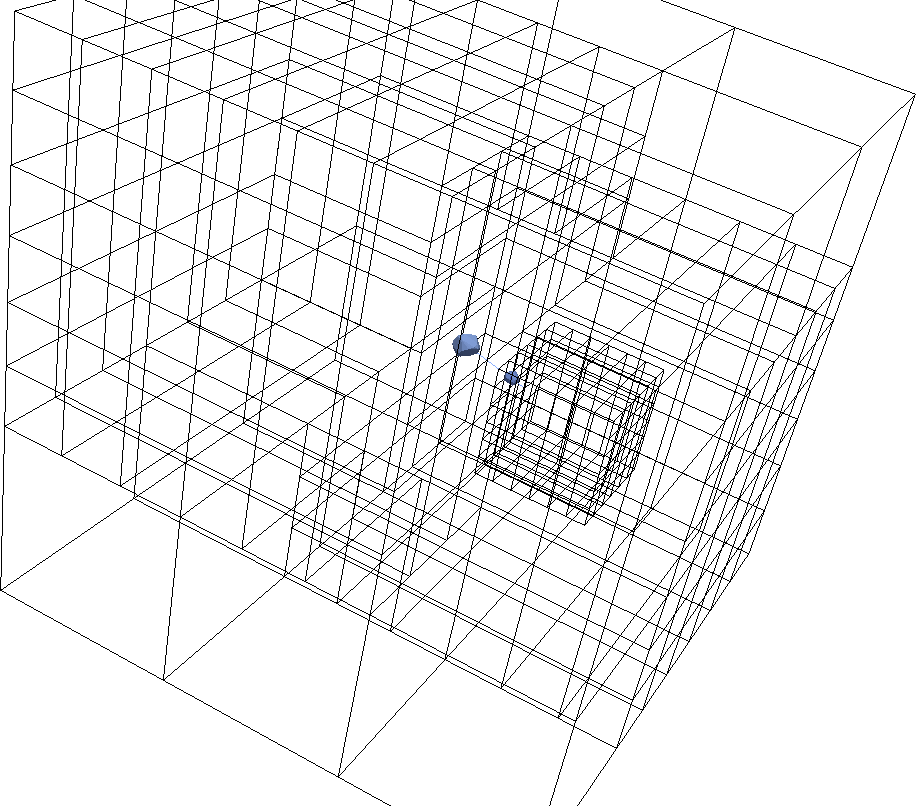
\includegraphics[width=0.3\textwidth]{experiments/two-bodies/visualisation/adaptive-grid01.png}
%   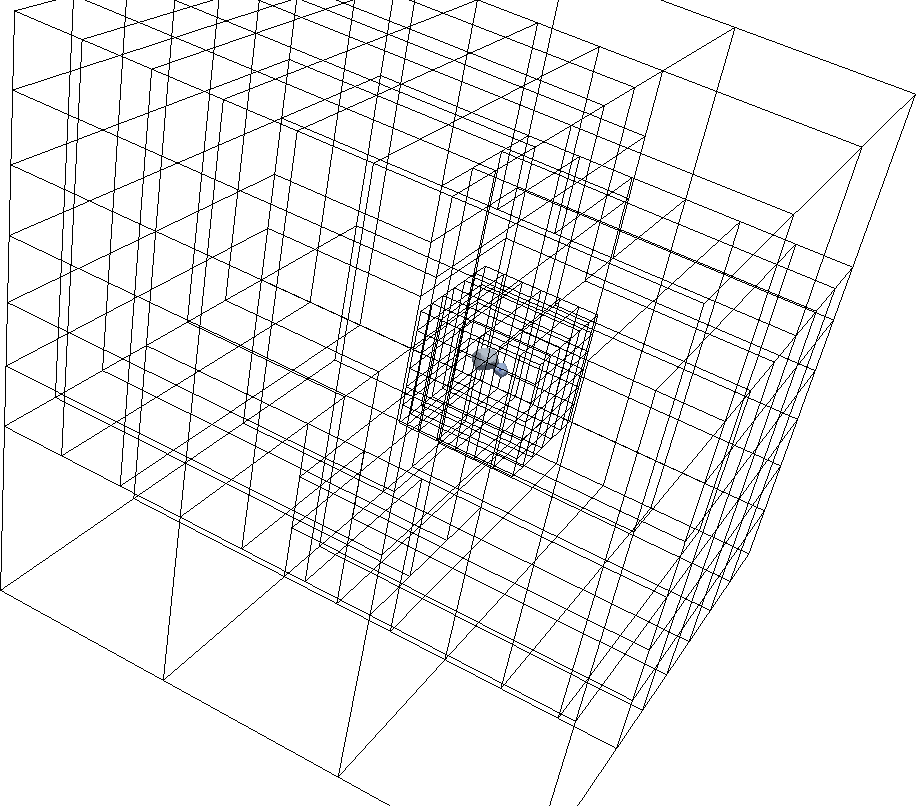
\includegraphics[width=0.3\textwidth]{experiments/two-bodies/visualisation/adaptive-grid02.png}
% \end{center}


{\bf Reluctant adaptive grid.} The reluctant adaptive grid behaves qualitatively
similar to the plain adaptive grid though yields quantitatively a smaller number
of vertices. 
We start from a grid with 498 vertices, i.e.~we do not refine the grid down to
the same fine level as the adaptive approach.
In iteration 6,334, both particles enter the same coarse grid cell and we run
3,944 triangle-triangle comparisions. 
They yield no contact yet.
The reluctant criterion refines the grid that has now 980 vertices starting from
iteration 6,338 on.
The code continues to run without any further comparisons till iteration 8,556
when the particles again are close to each other (close this time w.r.t.~finest
grid level allowed by the particle diameters).
Between iteration 8,557 and 9,533 we continue to run with 980 vertices and
3,944 comparisons.
The code decides to reduce the grid in iteration 9,536 to 747 vertices when the
particles are approach each other within a single cube that is resolved with a
fine grid.
We detects contact in iteration 9,541 after which the particles move away from
each other.
The 747 vertices are preserved and the code continues to run 3,944 comparisons.
In iteration 10,452, the particles are far away from each other. 
No more comparisons are performed from hereon.
In iteration 14,556 the particles are far away from each other, leave the
fine tessellation around the previous contact point and we continue with a
coarser grid of 498 vertices.

%  \begin{center}
%   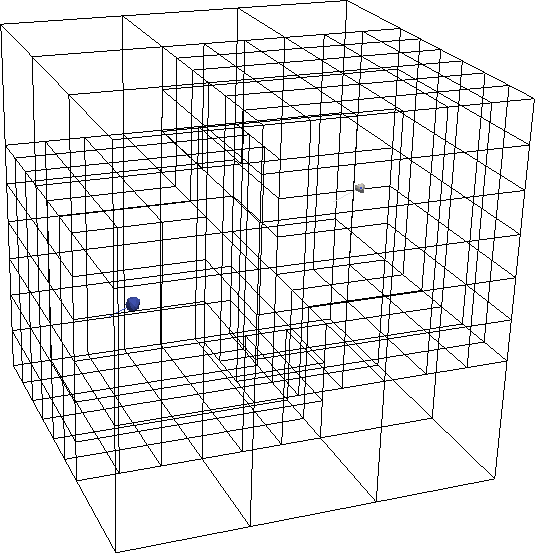
\includegraphics[width=0.3\textwidth]{experiments/two-bodies/visualisation/reluctant-adaptive-grid00.png}
%   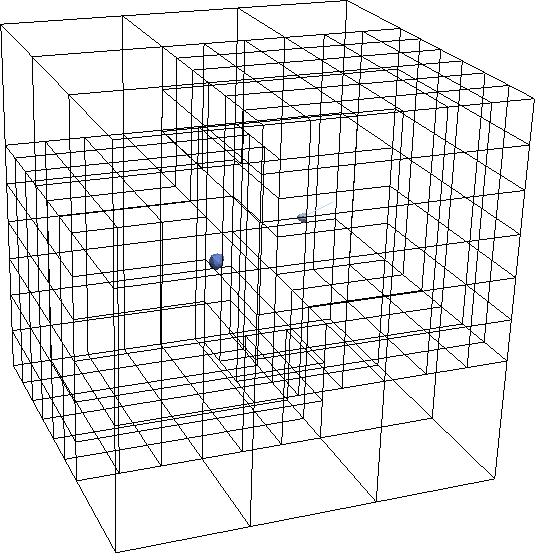
\includegraphics[width=0.3\textwidth]{experiments/two-bodies/visualisation/reluctant-adaptive-grid01.png}\\
%   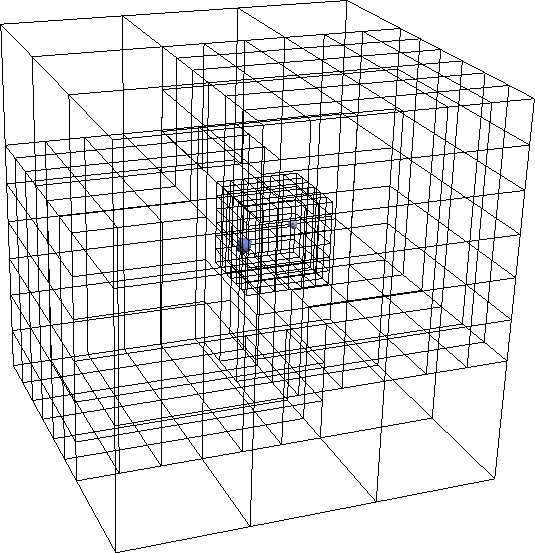
\includegraphics[width=0.3\textwidth]{experiments/two-bodies/visualisation/reluctant-adaptive-grid02.png}
%   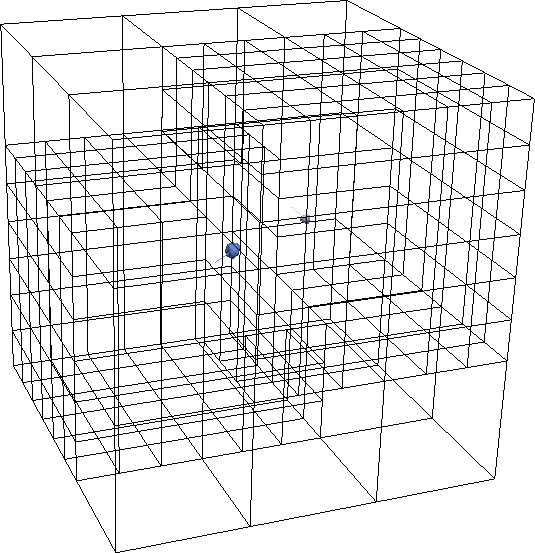
\includegraphics[width=0.3\textwidth]{experiments/two-bodies/visualisation/reluctant-adaptive-grid03.png}\\
%  \end{center}
